% !TeX program = pdfLaTeX
\documentclass[smallextended]{svjour3}       % onecolumn (second format)
%\documentclass[twocolumn]{svjour3}          % twocolumn
%
\smartqed  % flush right qed marks, e.g. at end of proof
%
\usepackage{amsmath}
\usepackage{graphicx}
\usepackage[utf8]{inputenc}

\usepackage[hyphens]{url} % not crucial - just used below for the URL
\usepackage{hyperref}

%
% \usepackage{mathptmx}      % use Times fonts if available on your TeX system
%
% insert here the call for the packages your document requires
%\usepackage{latexsym}
% etc.
%
% please place your own definitions here and don't use \def but
% \newcommand{}{}
%
% Insert the name of "your journal" with
% \journalname{myjournal}
%

%% load any required packages here



% tightlist command for lists without linebreak
\providecommand{\tightlist}{%
  \setlength{\itemsep}{0pt}\setlength{\parskip}{0pt}}

% From pandoc table feature
\usepackage{longtable,booktabs,array}
\usepackage{calc} % for calculating minipage widths
% Correct order of tables after \paragraph or \subparagraph
\usepackage{etoolbox}
\makeatletter
\patchcmd\longtable{\par}{\if@noskipsec\mbox{}\fi\par}{}{}
\makeatother
% Allow footnotes in longtable head/foot
\IfFileExists{footnotehyper.sty}{\usepackage{footnotehyper}}{\usepackage{footnote}}
\makesavenoteenv{longtable}

% Pandoc citation processing
\newlength{\cslhangindent}
\setlength{\cslhangindent}{1.5em}
\newlength{\csllabelwidth}
\setlength{\csllabelwidth}{3em}
\newlength{\cslentryspacingunit} % times entry-spacing
\setlength{\cslentryspacingunit}{\parskip}
% for Pandoc 2.8 to 2.10.1
\newenvironment{cslreferences}%
  {}%
  {\par}
% For Pandoc 2.11+
\newenvironment{CSLReferences}[2] % #1 hanging-ident, #2 entry spacing
 {% don't indent paragraphs
  \setlength{\parindent}{0pt}
  % turn on hanging indent if param 1 is 1
  \ifodd #1
  \let\oldpar\par
  \def\par{\hangindent=\cslhangindent\oldpar}
  \fi
  % set entry spacing
  \setlength{\parskip}{#2\cslentryspacingunit}
 }%
 {}
\usepackage{calc}
\newcommand{\CSLBlock}[1]{#1\hfill\break}
\newcommand{\CSLLeftMargin}[1]{\parbox[t]{\csllabelwidth}{#1}}
\newcommand{\CSLRightInline}[1]{\parbox[t]{\linewidth - \csllabelwidth}{#1}\break}
\newcommand{\CSLIndent}[1]{\hspace{\cslhangindent}#1}

\begin{document}


\title{Perdiz arrow points from Caddo burial contexts aid in defining
discrete behavioral regions \thanks{Components of the analytical
workflow were developed and funded by a Preservation Technology and
Training grant (P14AP00138) to RZS from the National Center for
Preservation Technology and Training, as well as grants to RZS from the
Caddo Nation of Oklahoma, National Forests and Grasslands in Texas
(15-PA-11081300-033) and the United States Forest Service
(20-PA-11081300-074). Additional financial and logistical support was
provided by the Heritage Research Center at Stephen F. Austin State
University.} }


    \titlerunning{Perdiz arrow points from Caddo burial contexts}

\author{  Robert Z. Selden 1 \and  John E. Dockall 2 \and  }

    \authorrunning{ Selden and Dockall }

\institute{
        Robert Z. Selden 1 \at
     Heritage Research Center, Stephen F. Austin State University;
Department of Biology, Stephen F. Austin State University; Texas
Archeological Research Laboratory, The University of Texas at Austin;
and Cultural Heritage Department, Jean Monnet University \\
     \email{\href{mailto:zselden@sfasu.edu}{\nolinkurl{zselden@sfasu.edu}}}  %  \\
%             \emph{Present address:} of F. Author  %  if needed
    \and
        John E. Dockall 2 \at
     Stantec, Inc. \\
     \email{\href{mailto:john.dockall@stantec.com}{\nolinkurl{john.dockall@stantec.com}}}  %  \\
%             \emph{Present address:} of F. Author  %  if needed
    \and
    }

\date{Received: date / Accepted: date}
% The correct dates will be entered by the editor


\maketitle

\begin{abstract}
Recent research into Caddo bottle and biface morphology yielded evidence
for two distinct behavioral regions, across which material culture from
Caddo burials expresses significant morphological differences. This
study asks whether Perdiz arrow points from Caddo burials differ across
the same geography, which would extend the pattern of morphological
differences to a third category of Caddo material culture. Perdiz arrow
points collected from the geographies of the northern and southern Caddo
behavioral regions were employed to test the hypothesis that
morphological attributes differ, and are predictable, between the two
communities. The analysis of linear metrics indicated a significant
difference in morphology by behavioral region. Using the linear metrics
combined with the tools of machine learning, a predictive
model---support vector machine---was designed to assess the degree to
which community differences could be predicted, achieving a receiver
operator curve score of 97 percent, and an accuracy score of 94 percent.
The subsequent landmark geometric morphometric analysis identified
significant differences in Perdiz arrow point shape and size between the
behavioral regions---one characterized by a comparatively smaller blade
and larger stem (north), and the other by a comparatively larger blade
and smaller stem (south)---coupled with significant results for
modularity and morphological integration. These findings build directly
upon recent investigations that posited two discrete Caddo behavioral
regions defined on the basis of discernible morphological differences,
which is expanded here to include a third category of Caddo material
culture.
\\
\keywords{
        American Southeast \and
        Caddo \and
        NAGPRA \and
        computational archaeology \and
        archaeoinformatics \and
        machine learning \and
        museum studies \and
        digital humanities \and
        non-Western art history \and
        STEM \and
        STEAM \and
    }


\end{abstract}


\def\spacingset#1{\renewcommand{\baselinestretch}%
{#1}\small\normalsize} \spacingset{1}


\hypertarget{intro}{%
\section{Introduction}\label{intro}}

Perdiz arrow points are considered the epitome of the Late Prehistoric
Toyah lithic assemblage in Texas---which also includes convex end
scrapers or unifaces, prismatic blades, as well as two- and four-beveled
bifacial knives---and are representative of the Late Prehistoric
transition to the Protohistoric (Arnn III 2012a). This technological
assemblage is typically attributed to groups of highly mobile bison
hunters, and has been documented across the geographic extent of Texas.
Our present understanding of the Toyah tool kit indicates that it was
successfully implemented in a broad-spectrum of hunting and foraging
lifeways that included not only bison (\emph{Bison bison}), but deer
(\emph{Odocoileus spp.}) and numerous other animal prey species (Arnn
III 2012a; Dering 2008).

The Toyah tool kit has been recognized as a potential contributor to
discussions of Late Prehistoric social and cultural identity. Initially
identified by J. Charles Kelley on the basis of technological and
morphological differences in material culture, the Toyah Phase (CE 1300
- 1700) occurrs between the Protohistoric and the preceding Austin Phase
of the Late Prehistoric Period (Kelley 1947a, 1947b). As noted by Arnn:

\begin{quote}
Toyah represents something of a paradox in which archaeologists have
identified \emph{one archaeological or material culture} in the same
region where historians have documented numerous Native American groups
and significant cultural diversity (Arnn III 2012a, 47).
\end{quote}

Stemming from the observations of Kelley, as well as later researchers
who viewed Toyah as a cultural entity, technological origins became a
point of further interest and debate from which two schools of thought
emerged regarding Toyah cultural manifestations: 1) that Toyah
represented the technology of Plains groups moving into Texas following
the bison herds (Prewitt 1981, 1985), or 2) a technocomplex or suite of
artifacts adopted by multiple groups across Texas as they participated
in bison hunting (Black 1986; Collins 1995; Ricklis 2017). In both
interpretations, primary agency is environmental (Arnn III 2012a);
either people followed the bison from elsewhere, or the influx of bison
spurred adoption of the technology among the numerous groups in Texas.

Research by Arnn (Arnn III 2005, 2007, 2012a, 2012b) emphasized aspects
of Toyah social identity, social fields, and agency, as well as the
archaeological visibility of these phenomena. Arnn recognized three
important scales of identity and interaction in his work:
community/band, marriage/linguistic group, and long-distance social
networks (Arnn III 2012a). His ideas are important here because they
supplant a simple monocausal environmental explanation of material
culture variability with a multi-causal and scaled concept that includes
social identity.

\hypertarget{perdiz-arrow-points}{%
\subsection{Perdiz arrow points}\label{perdiz-arrow-points}}

Perdiz arrow points generally follow two manufacturing
trajectories---one that enlists flakes, and the other, blade flakes
(Dockall et al. 2020; Johnson 1994; Ricklis 1994; Selden Jr et al.
2021)---and are known to encompass a greater range of variation in shape
and size than most arrow point types in Texas (Suhm and Jelks 1962;
Turner, Hester, and McReynolds 2011). Lithic tool stone in the ancestral
Caddo area of northeast Texas is relatively sparse (Selden Jr et al.
2021, fig. 2), consists primarily of chert, quartzite, and silicified
wood characteristic of the local geological formations, which may
contribute to local variation in shape and size (Selden Jr et al. 2021;
Banks 1990). It has been demonstrated elsewhere that the morphological
attributes of Perdiz arrow points from northeast Texas vary
significantly by time, raw material, and burial context (Selden Jr et
al. 2021). In outline, Perdiz arrow points possess a:

\begin{quote}
{[}t{]}riangular blade with edges usually quite straight but sometimes
slightly convex or concave. Shoulders sometimes at right angles to stem
but usually well barbed. Stem contracted, often quite sharp at base, but
may be somewhat rounded. Occasionally, specimen may be worked on one
face only or mainly on one face \ldots{} {[}w{]}orkmanship generally
good, sometimes exceedingly fine with minutely serrated blade edges
(Suhm, Krieger, and Jelks 1954, 504).
\end{quote}

A social network analysis of diagnostic artifacts from Historic Caddo
(post-CE 1680) sites in northeast Texas, which included Perdiz arrow
points, demonstrated two spatially discrete behavioral regions based
upon the co-presence of diagnostic types (Selden Jr. 2021a, fig. 12.4).
The network analysis was limited to Historic Caddo types; however,
Formative/Early Caddo (CE 800 -- 1200) Gahagan bifaces and Caddo bottle
types have been found to express significant morphological differences
across the same spatial extent as the behavioral regions (Selden Jr.
2018a, 2018b, 2019, 2021b), extending the prehistoric longevity for the
behavioral regions based on local alterity. Gahagan bifaces from the
ancestral Caddo area also differ significantly in shape, size, and form
compared with those recovered from central Texas sites (Selden Jr.,
Dockall, and Dubied 2020), suggesting a second shape boundary between
the ancestral Caddo area and central Texas.

\begin{figure}
\includegraphics[width=1\linewidth]{ms-figs/figure1} \caption{Location of Caddo sites with Perdiz arrow points used in this study, the extent of the ancestral Caddo area (white), and the Red River basin (blue), Sabine River basin (maroon), and Angelina River basin (brown).}\label{fig:fig1}
\end{figure}

The goal of this exploratory endeavor was to assess whether metrics
collected for Perdiz arrow points support the shape boundary posited in
recent social network and geometric morphometric analyses, to determine
whether linear metrics and shape variables might be useful predictors of
regional membership, and---if so---to identify those morphological
features that articulate with each behavioral region. Should the
analysis yield significant results, it would bolster the argument for at
least two discrete Caddo behavioral regions in northeast Texas; each
empirically defined by discernible morphological differences across
three discrete categories of Caddo material culture (Figure
\ref{fig:fig1}).

\hypertarget{caddo-behavioral-regions}{%
\subsection{Caddo behavioral regions}\label{caddo-behavioral-regions}}

In a June 18, 1937 Works Progress Administration interview with Lillian
Cassaway, Sadie Bedoka---a Caddo-Delaware woman raised with the
Caddo---stated that:

\begin{quote}
Each {[}Caddo{]} clan had its own shape to make its pottery. One clan
never thought of making anything the same pattern of another clan.
\emph{\textbf{You could tell who made the pottery by the shape}}
(Cassaway 1937, 395).
\end{quote}

General differences in Caddo ceramic forms have been noted elsewhere
(Krieger 1946; Selden Jr., Perttula, and O'Brien 2014); however, the
study of the Clarence H. Webb collection was the first to illustrate a
significant north-south geographic shape difference among Hickory
Engraved and Smithport Plain Caddo bottle types (Selden Jr. 2019). That
exploratory aperçu was later confirmed using more robust samples of
Hickory Engraved and Smithport Plain bottles (Selden Jr. 2018a, 2018b),
and was subsequently expanded to include a greater variety of Caddo
bottle types across a larger spatial and temporal extent (Selden Jr.
2021b).

The co-presence of diagnostic artifact and attribute types was leveraged
in defining Caddo phases and periods, which serve as a heuristic tool
that aids archaeologists in the explanation and retrojection of the
local cultural landscape, whilst simultaneously highlighting the
regional alterity that occurs between landscapes. The Historic Caddo
network expands those efforts, augmenting the previously-defined phases
and periods, and emphasizing the dynamic and manifold relational
connections that reinforce and transcend current epistemic categories
(Selden Jr. 2021a). This was achieved by enlisting a multi-scalar
methodological approach (Knappett 2011; Mills et al. 2015), where
northern and southern communities were parsed into constituent groups
using the co-presence of diagnostic types paired with a modularity
algorithm (Blondel et al. 2008; Lambiotte, Delvenne, and Barahona 2014).
Most constituent groups identified in the network analysis were found to
articulate with known Caddo polities (Selden Jr. 2021a).

A subsequent analysis of Gahagan bifaces confirmed that a second
category of Caddo material culture expressed significant morphological
differences across the same geography as the Hickory Engraved and
Smithport Plain bottles (Selden Jr., Dockall, and Shafer 2018). The
morphology of Gahagan bifaces from sites in central Texas has also been
found to differ significantly from those recovered from the Caddo region
(Selden Jr., Dockall, and Dubied 2020). That Gahagan bifaces were found
to differ across \emph{two} spatial boundaries was noteworthy,
particularly since it is regularly assumed that these large bifaces were
manufactured in central Texas and arrived in the ancestral Caddo area as
products of trade and/or exchange (Selden Jr., Dockall, and Dubied 2020;
Selden Jr., Dockall, and Shafer 2018). Further, that Gahagan bifaces
were found to differ across the same geography as those communities
posited in the Historic Caddo network analysis suggested that the
temporal range of the shape boundary might extend to the Formative/Early
Caddo period (CE 800 - 1250); a hypothesis that was later confirmed in a
more comprehensive analysis of Caddo bottles (Selden Jr. 2021b).

\hypertarget{methods-and-results}{%
\section{Methods and results}\label{methods-and-results}}

Sixty seven whole/intact Perdiz arrow points recovered from Caddo burial
contexts in Camp, Nacogdoches, and Shelby counties comprise the basis of
this study (\href{https://seldenlab.github.io/perdiz3/}{supplementary
materials}). A standard suite of linear metrics were collected for each
specimen, including maximum length, width, thickness, stem length, and
stem width (Table @ref\{tab:table1\}). Following collection, data were
imported to R (Team 2021), where boxplots were produced, along with a
principal components analysis (PCA), followed by a permutational
multivariate analysis of variance (perMANOVA) to test whether the
morphology of Perdiz arrow points differs between the behavioral regions
(\href{https://seldenlab.github.io/perdiz3/}{supplementary materials}).

\begin{longtable}[]{@{}lccccccc@{}}
\caption{Sample overview: Linear metrics and categorical variables used
in the study, which include maximum length (MaxL), width (MaxW),
thickness (MaxTh), stem length (MaxStL), and stem width
(MaxStW).}\tabularnewline
\toprule()
ID & Site & Region & MaxL & MaxW & MaxTh & MaxStl & MaxStw \\
\midrule()
\endfirsthead
\toprule()
ID & Site & Region & MaxL & MaxW & MaxTh & MaxStl & MaxStw \\
\midrule()
\endhead
554 & 41cp12 & north & 25.40 & 12.18 & 3.82 & 5.75 & 3.84 \\
555 & 41cp12 & north & 22.92 & 12.87 & 3.54 & 3.71 & 3.69 \\
556 & 41cp12 & north & 24.09 & 11.87 & 3.61 & 5.15 & 4.78 \\
559 & 41cp12 & north & 25.01 & 10.57 & 3.50 & 5.84 & 3.88 \\
562 & 41cp12 & north & 22.10 & 10.45 & 3.47 & 3.77 & 3.43 \\
565 & 41cp12 & north & 20.31 & 10.53 & 3.08 & 2.01 & 3.07 \\
591 & 41cp12 & north & 25.49 & 13.37 & 4.42 & 7.04 & 4.95 \\
646 & 41cp5 & north & 16.37 & 10.46 & 2.63 & 3.85 & 4.03 \\
649 & 41cp5 & north & 23.38 & 13.88 & 4.11 & 7.33 & 5.54 \\
651 & 41cp5 & north & 22.86 & 13.84 & 4.61 & 6.16 & 5.02 \\
652 & 41cp5 & north & 22.51 & 12.67 & 3.37 & 6.33 & 4.39 \\
653 & 41cp5 & north & 27.55 & 17.05 & 3.08 & 6.83 & 4.60 \\
654 & 41cp5 & north & 17.01 & 10.90 & 2.35 & 4.64 & 3.64 \\
655 & 41cp5 & north & 26.86 & 13.06 & 2.50 & 6.10 & 3.99 \\
656 & 41cp5 & north & 25.79 & 12.52 & 2.96 & 5.43 & 3.97 \\
657 & 41cp5 & north & 27.36 & 12.41 & 3.04 & 6.56 & 4.26 \\
659 & 41cp5 & north & 23.10 & 11.42 & 2.14 & 4.74 & 4.21 \\
660 & 41cp5 & north & 20.23 & 9.64 & 1.89 & 5.70 & 2.66 \\
661 & 41cp5 & north & 21.73 & 10.67 & 2.27 & 4.91 & 3.13 \\
665 & 41cp12 & north & 27.34 & 15.77 & 4.10 & 4.69 & 4.60 \\
677 & 41cp20 & north & 24.72 & 13.70 & 2.52 & 6.98 & 3.76 \\
678 & 41cp20 & north & 24.98 & 13.33 & 3.26 & 4.19 & 3.54 \\
na49-1 & 41na49 & south & 47.74 & 15.14 & 4.52 & 6.82 & 6.22 \\
na49-10 & 41na49 & south & 22.88 & 12.13 & 3.68 & 5.73 & 5.49 \\
na49-11 & 41na49 & south & 24.09 & 12.52 & 3.27 & 5.36 & 4.81 \\
na49-12 & 41na49 & south & 21.41 & 10.31 & 3.48 & 4.64 & 3.82 \\
na49-13 & 41na49 & south & 24.84 & 11.21 & 3.51 & 5.19 & 4.97 \\
na49-14 & 41na49 & south & 21.92 & 9.35 & 2.62 & 5.22 & 4.85 \\
na49-2 & 41na49 & south & 32.49 & 12.78 & 3.80 & 6.80 & 4.78 \\
na49-3 & 41na49 & south & 27.72 & 13.05 & 4.19 & 5.99 & 5.88 \\
na49-4 & 41na49 & south & 26.20 & 10.60 & 3.30 & 4.67 & 4.92 \\
na49-7 & 41na49 & south & 24.25 & 12.01 & 2.92 & 6.01 & 4.93 \\
na49-8 & 41na49 & south & 22.06 & 14.51 & 2.92 & 5.67 & 5.17 \\
na49-9 & 41na49 & south & 25.44 & 13.86 & 3.44 & 4.74 & 4.81 \\
f2-g2-5 & 41sy27 & south & 24.92 & 16.16 & 3.57 & 4.44 & 4.25 \\
f2-g2-10 & 41sy27 & south & 34.69 & 16.40 & 3.29 & 6.12 & 4.14 \\
f2-g2-15 & 41sy27 & south & 34.17 & 20.00 & 3.09 & 8.34 & 5.68 \\
f2-g2-9 & 41sy27 & south & 39.39 & 16.73 & 2.95 & 6.28 & 4.90 \\
f2-g2-14 & 41sy27 & south & 30.36 & 15.72 & 2.58 & 6.11 & 4.51 \\
f2-g2-2 & 41sy27 & south & 29.32 & 15.47 & 2.94 & 5.59 & 4.18 \\
f2-g2-1 & 41sy27 & south & 30.83 & 16.80 & 2.96 & 5.83 & 5.21 \\
f2-g2-11 & 41sy27 & south & 31.10 & 15.33 & 2.92 & 5.60 & 4.78 \\
f2-g2-3 & 41sy27 & south & 23.30 & 15.31 & 3.09 & 3.87 & 4.31 \\
f2-g2-13 & 41sy27 & south & 29.33 & 18.59 & 3.13 & 5.54 & 4.52 \\
f2-g2-7 & 41sy27 & south & 24.78 & 15.68 & 3.20 & 4.60 & 4.23 \\
f2-g2-8 & 41sy27 & south & 28.17 & 18.24 & 3.01 & 5.99 & 4.72 \\
f2-g2-12 & 41sy27 & south & 33.53 & 15.83 & 3.18 & 5.55 & 4.23 \\
f2-g2-6 & 41sy27 & south & 23.74 & 16.12 & 2.92 & 5.53 & 4.34 \\
f2-g1-20 & 41sy27 & south & 37.46 & 16.78 & 3.28 & 7.53 & 5.54 \\
f2-g1-10 & 41sy27 & south & 27.32 & 18.39 & 3.10 & 5.37 & 4.54 \\
f2-g1-19 & 41sy27 & south & 31.44 & 19.62 & 3.13 & 5.44 & 5.75 \\
f2-g1-17 & 41sy27 & south & 32.75 & 19.34 & 3.34 & 6.29 & 5.31 \\
f2-g1-16 & 41sy27 & south & 34.97 & 16.81 & 3.39 & 5.90 & 5.49 \\
f2-g1-11 & 41sy27 & south & 33.18 & 17.45 & 3.36 & 6.47 & 5.12 \\
f2-g1-13 & 41sy27 & south & 31.61 & 18.57 & 3.07 & 5.75 & 5.04 \\
f2-g1-15 & 41sy27 & south & 38.50 & 20.34 & 3.40 & 8.85 & 6.16 \\
f2-g1-18 & 41sy27 & south & 30.02 & 17.33 & 3.21 & 7.05 & 5.18 \\
f2-g1-3 & 41sy27 & south & 29.45 & 18.84 & 3.16 & 5.58 & 5.32 \\
f2-g1-7 & 41sy27 & south & 32.44 & 18.20 & 3.28 & 5.80 & 4.76 \\
f2-g1-4 & 41sy27 & south & 28.33 & 17.49 & 2.98 & 7.29 & 4.83 \\
f2-g1-12 & 41sy27 & south & 32.17 & 18.47 & 3.47 & 5.44 & 5.20 \\
f2-g1-8 & 41sy27 & south & 31.03 & 17.05 & 3.10 & 7.41 & 5.11 \\
f2-g1-9 & 41sy27 & south & 27.56 & 21.12 & 3.47 & 6.84 & 5.07 \\
f2-g3-1 & 41sy27 & south & 27.21 & 17.41 & 3.52 & 7.70 & 5.35 \\
f2-g3-3 & 41sy27 & south & 24.31 & 16.35 & 3.00 & 7.08 & 5.10 \\
f2-g3-6 & 41sy27 & south & 30.58 & 18.03 & 3.56 & 7.37 & 4.81 \\
f2-g3-2 & 41sy27 & south & 27.63 & 17.74 & 2.99 & 8.23 & 4.82 \\
\bottomrule()
\end{longtable}

Boxplots illustrate the distribution and mean for each of the five
linear variables (Figure \ref{fig:fig2}a-e), and the PCA (Figure
\ref{fig:fig2}f) illustrates over 92 percent of the variation in the
sample among PC1 (84.65 percent) and PC2 (11.71 percent). The perMANOVA
demonstrated that linear metrics for Perdiz arrow points differ
significantly by behavioral region (permutations = 10,000; Rsq =
0.29485; Pr(\textgreater F) = 1e-04)
(\href{https://seldenlab.github.io/perdiz3/}{supplementary materials}).

\begin{figure}
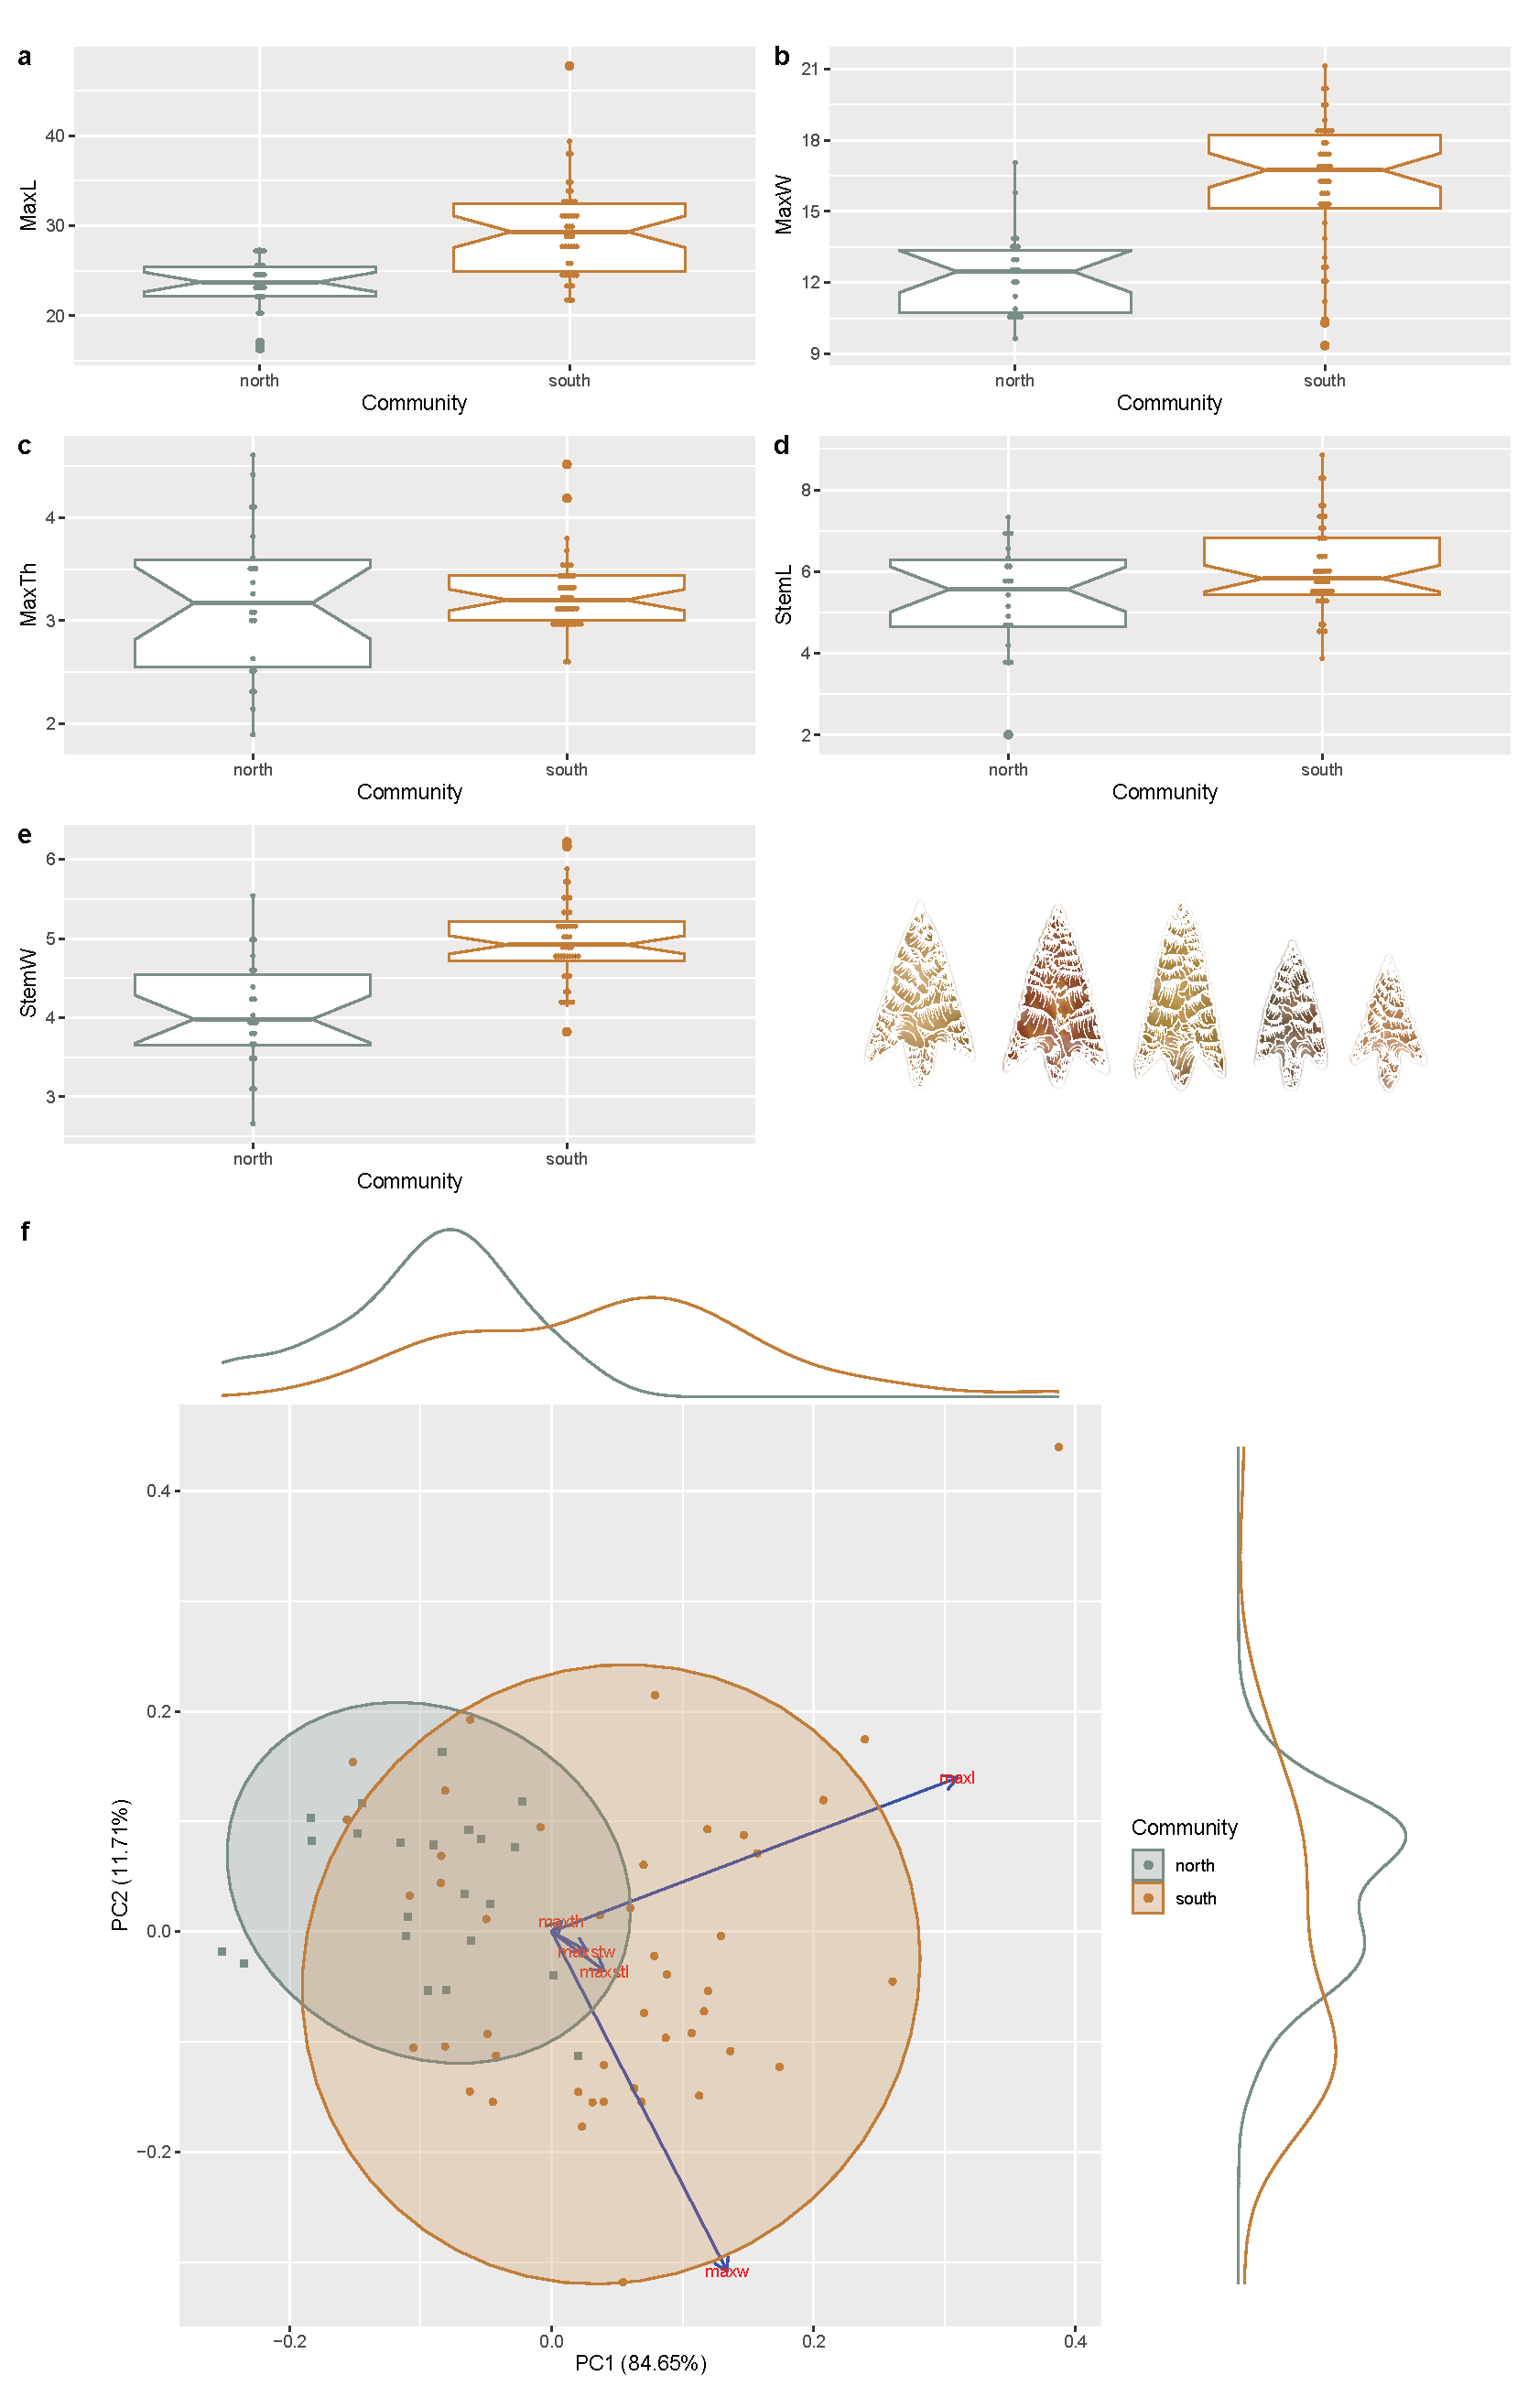
\includegraphics[width=0.95\linewidth]{ms-figs/figure2} \caption{Boxplots for a, maximum length; b, maximum width; c, maximum thickness; d, stem length; e, stem width, and f, PCA [on correlation matrix] for linear metrics associated with the Perdiz arrow points. Additional information related to the analysis, including all linear data and the code needed to reproduce these results, can be found in the supplemental materials at https://seldenlab.github.io/perdiz3/.}\label{fig:fig2}
\end{figure}

\hypertarget{predictive-model}{%
\subsection{Predictive model}\label{predictive-model}}

A \emph{support vector machine} is a supervised machine learning model
regularly used in classifying archaeological materials (Bhatt and
Patalia 2017; Monna et al. 2020; Febriawan et al. 2020; Kadhim and Abed
2021; Zhang 2013; Elliot et al. 2021), which has utility in comparing
and classifying datasets aggregated from digital repositories,
comparative collections, open access reports, as well as other digital
assets. For this effort, linear data were imported and modeled using the
\texttt{scikit-learn} package in Python (Pedregosa et al. 2011; Buitinck
et al. 2013) (\href{https://seldenlab.github.io/perdiz3/}{supplementary
materials}), and subsequently split into training (75 percent) and
testing (25 percent) subsets. A standard scaler was used to decrease the
sensitivity of the algorithm to outliers by standardizing features, and
a nested cross validation of the training set was used to achieve
unbiased estimates of model performance, resulting in a mean cross
validation score of 86 percent
(\href{https://seldenlab.github.io/perdiz3/}{supplementary materials}).
The model was subsequently fit on the training set, yielding a receiver
operator curve score of 97 percent, and an accuracy score of 94 percent
(\href{https://seldenlab.github.io/perdiz3/}{supplementary materials}).

\hypertarget{geometric-morphometrics}{%
\subsection{Geometric morphometrics}\label{geometric-morphometrics}}

Each of the arrow points was imaged using a flatbed scanner (HP Scanjet
G4050) at 600 dpi. The landmarking protocol developed for this study
(\href{https://seldenlab.github.io/perdiz3/}{supplementary materials})
included six landmarks and 24 equidistant semilandmarks to characterize
Perdiz arrow point shape, and were applied using the
\texttt{StereoMorph} package in R (Olsen and Westneat 2015). The
characteristic points and tangents used in the landmarking protocol were
inspired by the work of Birkhoff (Birkhoff 1933).

Landmarks were aligned to a global coordinate system (Kendall 1981,
1984; Slice 2001), achieved through generalized Procrustes
superimposition (Rohlf and Slice 1990), performed in R 4.1.1 (Team 2021)
using the \texttt{geomorph} package v4.0.1 (Dean C. Adams and
Otarola-Castillo 2013; Baken et al. 2021) (Figure \ref{fig:fig3}).
Procrustes superimposition translates, scales, and rotates the
coordinate data allowing for comparisons among objects (Gower 1975;
Rohlf and Slice 1990). The \texttt{geomorph} package uses a partial
Procrustes superimposition that projects the aligned specimens into
tangent space subsequent to alignment in preparation for the use of
multivariate methods that assume linear space Slice (2001).

\begin{figure}
\includegraphics[width=0.95\linewidth]{ms-figs/figure3} \caption{Results of generalized Procrustes analysis, illustrating mean shape (black) and all specimens in the sample (gray), as well as the difference in centroid size for Perdiz arrow points from the two behavioral regions. Additional information related to the GPA, including all data and code needed to reproduce these results, can be found in the supplemental materials at https://seldenlab.github.io/perdiz3/.}\label{fig:fig3}
\end{figure}

Principal components analysis (Jolliffe 2002; Revell 2009) was used to
visualize shape variation among the arrow points (Figure
\ref{fig:fig4}). Shape changes described by each principal axis are
commonly visualized using thin-plate spline warping of a reference image
or 3D mesh (Klingenberg 2013; Sherratt et al. 2014). A residual
randomization permutation procedure (RRPP; n = 10,000 permutations) was
used for all Procrustes ANOVAs (Dean C. Adams and Collyer 2015; Michael
L. Collyer and Adams 2018), which has higher statistical power and a
greater ability to identify patterns in the data should they be present
(Anderson and Ter Braak 2003). To assess whether shape differs by group
(region), Procrustes ANOVAs (Goodall 1991) were also run that enlist
effect-sizes (z-scores) computed as standard deviates of the generated
sampling distributions (M. L. Collyer, Sekora, and Adams 2015).
Procrustes variance was used to discriminate between regions and compare
the amount of shape variation (morphological disparity) (Zelditch et al.
2004), estimated as Procrustes variance using residuals of linear model
fit (Dean C. Adams et al. 2018). A pairwise comparison of morphological
integration was used to test the strength of integration between blade
and basal morphology using a z-score (Bookstein et al. 2003; M. L.
Collyer, Sekora, and Adams 2015; Dean C. Adams and Collyer 2016; D. C.
Adams and Collyer 2019).

\begin{figure}
\includegraphics[width=1\linewidth]{ms-figs/figure4} \caption{Principal components analysis plot (PC1/PC2) for Perdiz arrow points by behavioral region/community (top; gray squares, north; orange triangles, south), and results of modularity (bottom left) and blade/base morphological integration (bottom right) analyses. Additional information related to the PCA, including the full listing of results and all data and code needed to reproduce these results, can be found in the supplemental materials at https://seldenlab.github.io/perdiz3/.}\label{fig:fig4}
\end{figure}

A Procrustes ANOVA was used to test for a difference in Perdiz arrow
point (centroid) size by behavioral region (RRPP = 10,000; Rsq =
0.30681; Pr(\textgreater F) = 1e-04), followed by a second to test for a
difference in arrow point shape (RRPP = 10,000; Rsq = 0.0536;
Pr(\textgreater F) = 0.0161). While shape and size differ significantly
between behavioral regions, the Rsq value for size is just under six
times larger than that for shape (smaller in the north; larger in the
south), suggesting that between-region differences in Perdiz arrow point
\emph{size} may be more visually apparent than differences in
\emph{shape}. A comparison of mean consensus configurations was used to
illustrate shape differences from the northern and southern behavioral
regions. Diacritical morphology is characterized by a comparatively
smaller blade and larger stem in the north, and by a comparatively
larger blade and smaller stem in the south. Further, the angle between
the shoulder and base is more acute, with a base that is generally
shorter and narrower in the southern behavioral region
(\href{https://seldenlab.github.io/perdiz3/}{supplementary materials}).

The analysis of modularity, which compares within-module covariation of
landmarks against between-module covariation was significant (see Figure
\ref{fig:fig4} and
\href{https://seldenlab.github.io/perdiz3/}{supplementary materials})
(D. C. Adams and Collyer 2019; Dean C. Adams and Peres-Neto 2016),
demonstrating that Perdiz arrow point blades and bases are, in fact,
modular. The test for morphological integration was also significant
(see Figure \ref{fig:fig4} and
\href{https://seldenlab.github.io/perdiz3/}{supplementary materials}),
indicating that the blades and bases of Perdiz arrow points are
integrated. These results demonstrate that blade and base shapes for
Perdiz arrow points are predictable; a finding that would have utility
in subsequent studies of Perdiz arrow point morphology that incorporate
fragmentary specimens.

\hypertarget{discussion}{%
\section{Discussion}\label{discussion}}

The shape boundary empirically delineates two discrete behavioral
regions in the ancestral Caddo area. That Perdiz arrow points recovered
from Caddo burials north and south of the shape boundary were found to
differ significantly, expands the scope of the behavioral regions to
include three classes of material culture (Caddo bottles, bifaces,
and---now---arrow points) (Selden Jr. 2018a, 2018b, 2019, 2021b; Selden
Jr., Dockall, and Dubied 2020; Selden Jr., Dockall, and Shafer 2018;
Selden 2022). Thus, for material culture included in burial contexts
north and south of the shape boundary, the Caddo were selecting for
significant morphological differences in bottles, bifaces, and arrow
points (Figure \ref{fig:fig6}a-d). Results clearly illustrate that
morphological differences among Perdiz arrow points found in the
northern and southern behavioral regions (Figure \ref{fig:fig6}d) are
predictable (\href{https://seldenlab.github.io/perdiz3/}{supplementary
materials}), and can be disaggregated using a standard suite of linear
metrics regularly collected in the course of cultural resource
management endeavors.

\begin{figure}
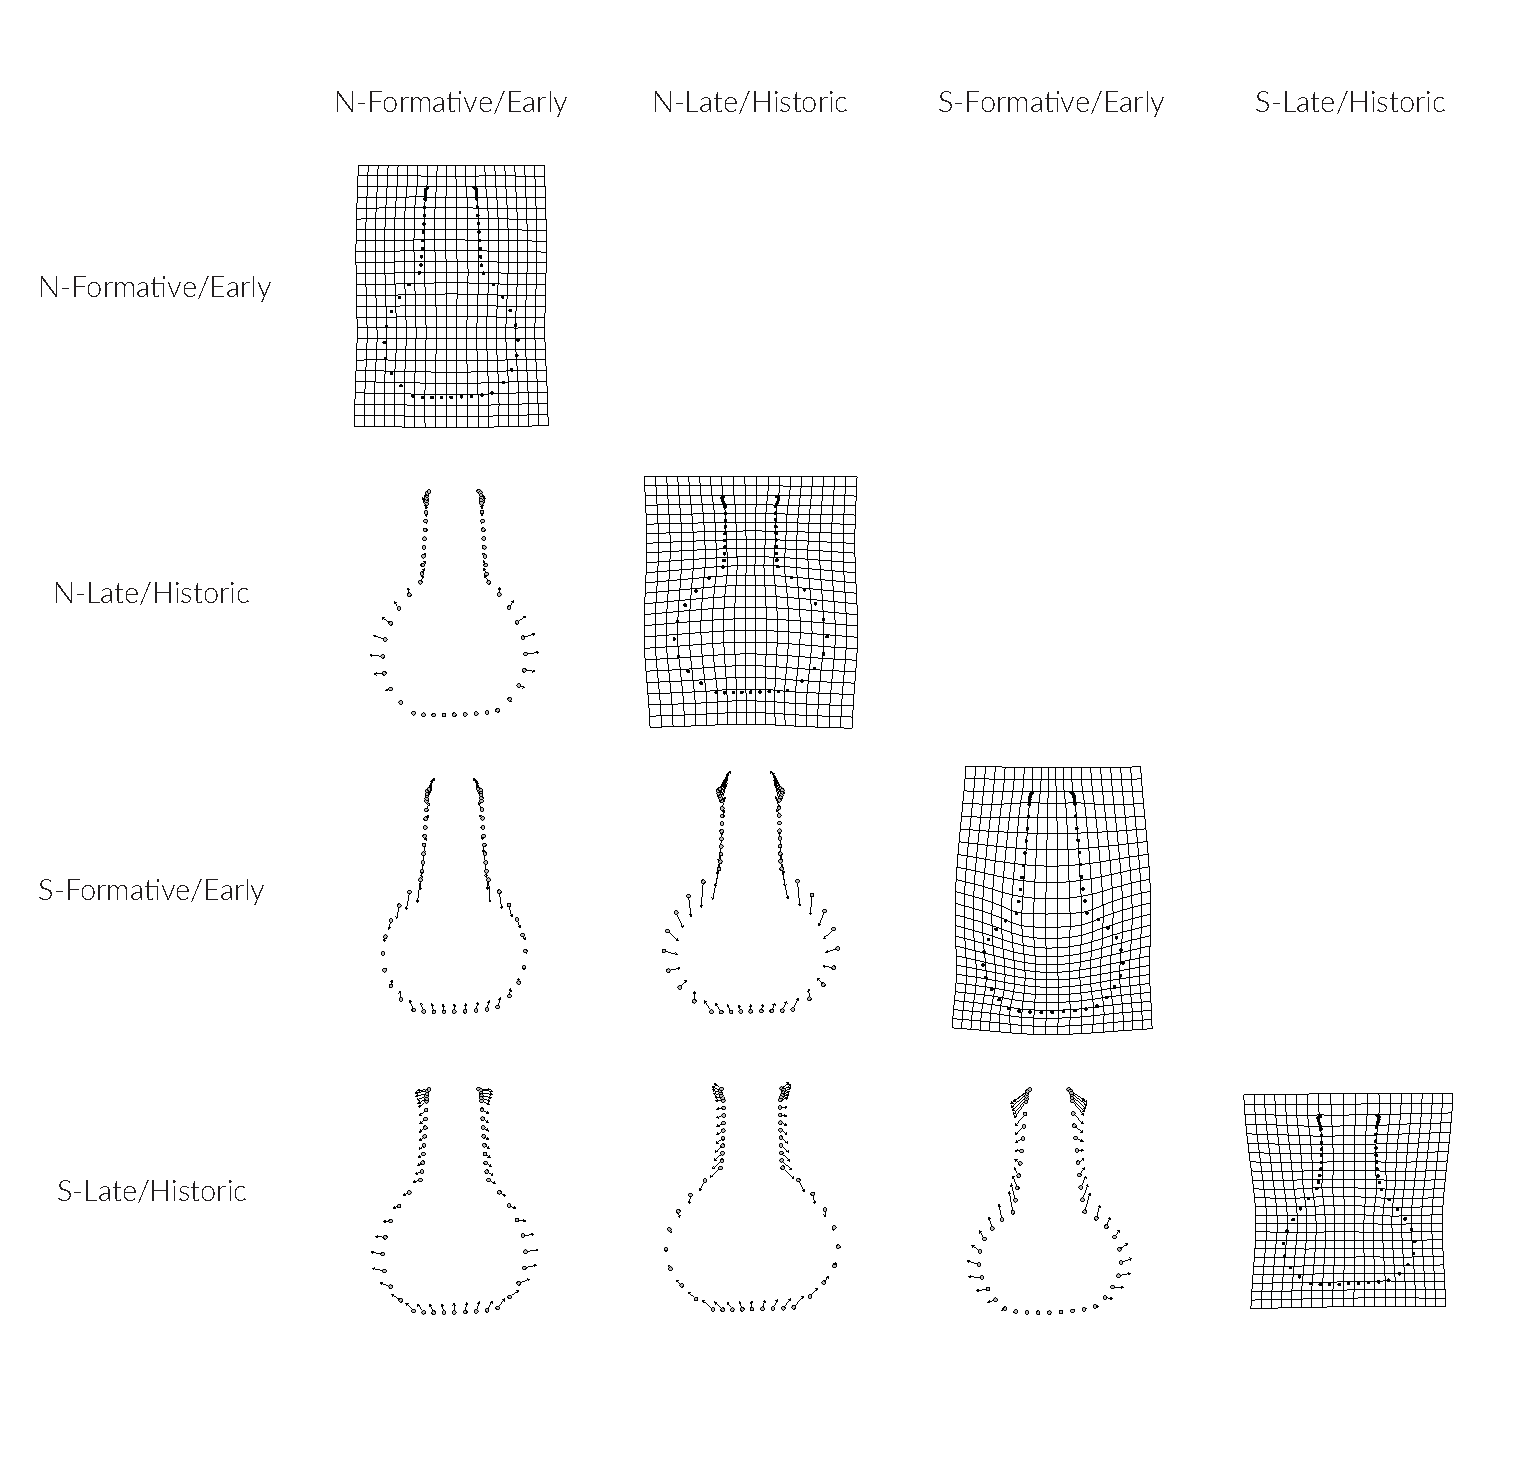
\includegraphics[width=1\linewidth]{ms-figs/figure6} \caption{Mean shapes and comparisons for a, Formative/Early and b, Late/Historic bottles; c, Formative/Early Gahagan bifaces; and d, Middle/Late Perdiz arrow points from Caddo burial contexts in the northern and southern behavioral regions. In the comparisons of mean shape, the northern population appears in gray, and the southern population appears in black.}\label{fig:fig6}
\end{figure}

The geometric morphometric analysis demonstrated significant
morphological differences for Perdiz arrow points recovered north and
south of the shape boundary, where the most pronounced difference was
found to occur in basal morphology (see Figure \ref{fig:fig6}d). This
finding provides evidence in support of the argument that Perdiz arrow
point morphology is labile (Selden Jr et al. 2021). The character of
those morphological differences found to occur in Perdiz arrow points
(basal morphology and size) is potentially suggestive of differential
approaches to hafting.

Blades and bases of Perdiz arrow points were found to be both modular
and morphologically integrated. This indicates that each module
functions independently, and that basal shape is a predictor of blade
shape, and vice-versa. Further work is warranted to assess whether
Perdiz arrow points from groups within the boundaries of the northern
and southern behavioral regions may express unique morphologies, aiding
in further delimiting local boundaries associated with constituent Caddo
groups.

\hypertarget{morphologically-distinct-behavioral-regions}{%
\subsection{Morphologically-distinct behavioral
regions}\label{morphologically-distinct-behavioral-regions}}

In considering the role/s of material culture as aspects of social
identity, it is important not to lose sight of the fact that people and
their possessions are active agents in the production and maintenance of
social identity/ies. All three categories of material culture (bottles,
bifaces, and arrow points) contribute to local and regional communities
of identity and communities of practice (Eckert, Schleher, and James
2015). Generally, this concept may be more easily applied to bottles
since those were manufactured and used by individuals sharing collective
Caddo identities. Bifaces and arrow points potentially represent
multiple identities---those being the Caddo, as users; and non-Caddo, as
producers---at least with regard to chipped stone tools incorporated in
mortuary contexts. This concept lends defensible credence to the notion
of morphologically-distinct behavioral regions among the Caddo, while
integrating the possibility of understanding interactions between Caddo
and non-Caddo groups, to include the movement of material culture
between Caddo behavioral regions.

Three categories of Caddo material culture have been demonstrated to
differ north and south of the shape boundary, indicating a haecceity of
regional perspectives related to production (bottles), and aesthetic
choice/cultural interaction (bifaces and arrow points). These differing
perspectives incorporate normative group decisions that include shape,
size, form, and decorative expression, which likely represent the
culmination of generational perspectives (Stark 2006). Simply stated,
such perspectives are representative of tradition. Eckert and colleagues
(Eckert, Schleher, and James 2015) indicate that provenance, the origin
or source of an item, is a significant component of understanding the
interrelatedness of communities of identity and communities of practice.
A second shape boundary demonstrates that Gahagan bifaces differ
significantly between the ancestral Caddo region and central Texas,
where they are currently thought to have been manufactured. This
suggests that those communities of practice that articulate with the
\emph{production} of chipped stone artifacts recovered from Caddo
internments, may not have been Caddo.

It is also entirely possible that there are no communities of practice
for chipped stone artifacts recovered from Caddo mortuary contexts.
However, there do appear to have been communities of practice associated
with Perdiz arrow points recovered from non-mortuary contexts in the
ancestral Caddo area, which may more readily reflect retouch or
resharpening approaches used by Caddo knappers (Selden Jr et al. 2021;
Shafer 1974; Selden 2022). Similar interpretations can be applied to the
Gahagan bifaces, as few have been reported outside of Caddo mortuary
contexts. It may be more fitting to perceive of Perdiz arrow points and
Gahagan bifaces as indicative of communities of identity rather than
communities of practice, due to the contextual discrepancy evinced
through mortuary and non-mortuary settings. The provenance of bifaces
from Caddo mortuary contexts can most assuredly be considered non-local,
or produced outside of the ancestral Caddo region, based on multiple
factors that include raw material, workmanship, morphology, and context.

\hypertarget{conclusion}{%
\section{Conclusion}\label{conclusion}}

This study demonstrated that linear metrics and shape variables
collected for Perdiz arrow points support the shape boundary posited in
recent social network and geometric morphometric analyses, and
determined that those same metrics can be used to predict regional
membership. Morphological features that discriminate between Perdiz
arrow points recovered from each behavioral region were identified using
geometric morphometrics, with substantive differences found to occur in
size and basal morphology. Blade and base shape were found to be both
modular and morphologically integrated, suggesting that blade and base
shapes are predictable. While evidence from one category---Caddo
bottles---supports discussions of Caddo production, the other
two---bifaces and arrow points---may articulate with production
activities outside of the region by non-Caddo makers. Such production
activity is more likely to be localized than exchange systems, thus
assumed to leave a clearer signature (Costin 1991).

\hypertarget{acknowledgments}{%
\section{Acknowledgments}\label{acknowledgments}}

We extend our gratitude to the Caddo Nation of Oklahoma, the Caddo
Nation Tribal Council, Tribal Chairman, and Tribal Historic Preservation
Office for their continued guidance and support of our work, as well as
access to NAGPRA and previously repatriated collections. Thanks also to
the Anthropology and Archaeology Laboratory at Stephen F. Austin State
University for the requisite permissions and access to the NAGPRA
objects from the Washington Square Mound site and Turner collections,
and to Tom A. Middlebrook for brokering access to the Perdiz arrow
points from burials at the Morse Mound site. We wish to thank Michael J.
Shott and Casey Wayne Riggs for their useful comments and constructive
criticisms on a presubmission draft, and extend our gratitude to Emma
Sherratt, Kersten Bergstrom, Lauren Butaric, Julien Claude, Dean C.
Adams, and Michael L. Collyer for their constructive criticisms and
suggestions throughout the development of this research program.
Additional comments from the editor and three anonymous reviewers aided
in further refining the manuscript.

\hypertarget{funding}{%
\section{Funding}\label{funding}}

Components of the analytical workflow were developed and funded by a
Preservation Technology and Training grant (P14AP00138) to RZS from the
National Center for Preservation Technology and Training, as well as
grants to RZS from the Caddo Nation of Oklahoma, National Forests and
Grasslands in Texas (15-PA-11081300-033) and the United States Forest
Service (20-PA-11081300-074). Additional funding and logistical support
was provided by the Heritage Research Center at Stephen F. Austin State
University.

\hypertarget{data-management}{%
\section{Data Management}\label{data-management}}

The data and analysis code associated with this project can be accessed
through the GitHub repository
(\url{https://github.com/seldenlab/perdiz3}) or the supplementary
materials (\url{https://seldenlab.github.io/perdiz3/}); which are
digitally curated on the Open Science Framework \newline 
(\href{https://osf.io/vzhjr/}{DOI: 10.17605/OSF.IO/VZHJR}). Images of
all Perdiz arrow points used in this study were made available in an
open access comparative collection
(\url{https://scholarworks.sfasu.edu/ita-perdiz/}), with permission from
the Caddo Nation of Oklahoma. These supplementary materials include all
analysis data and code used in the study, providing a means for others
to reproduce (exactly) those results discussed and expounded upon in
this article. The replicable nature of this undertaking provides others
with the means to critically assess and evaluate the various analytical
components of this study, which is a necessary requirement for the
production of reliable knowledge (Gray and Marwick 2019; Peng 2011;
Gandrud 2014).

Reproducibility projects in \href{https://osf.io/ezcuj/}{psychology} and
\href{https://www.cos.io/rpcb}{cancer biology} are impacting current
research practices across all domains. Examples of reproducible research
are becoming more abundant in archaeology (Marwick 2016; Ivanovaitė et
al. 2020; Selden Jr., Dockall, and Dubied 2020; Selden Jr et al. 2021;
Selden 2022), and the next generation of archaeologists are learning
those tools and methods needed to reproduce and/or replicate research
results (Marwick et al. 2019). Reproducible and replicable research work
flows are often employed at the highest levels of humanities-based
inquiries to mitigate concern or doubt regarding proper execution, and
is of particular import should the results have---explicitly or
implicitly---a major impact on scientific progress (Peels and Bouter
2018).

\hypertarget{references-cited}{%
\section*{References cited}\label{references-cited}}
\addcontentsline{toc}{section}{References cited}

\hypertarget{refs}{}
\begin{CSLReferences}{1}{0}
\leavevmode\vadjust pre{\hypertarget{ref-RN10874}{}}%
Adams, D. C., and M. L. Collyer. 2019. {``Comparing the Strength of
Modular Signal, and Evaluating Alternative Modular Hypotheses, Using
Covariance Ratio Effect Sizes with Morphometric Data.''} Journal
Article. \emph{Evolution} 73 (12): 2352--67.
\url{https://doi.org/10.1111/evo.13867}.

\leavevmode\vadjust pre{\hypertarget{ref-RN8579}{}}%
Adams, Dean C., and Michael L. Collyer. 2015. {``{Permutation Tests for
Phylogenetic Comparative Analyses of High-Dimensional Shape Data: What
you Shuffle Matters}.''} Journal Article. \emph{Evolution} 69 (3):
823--29. \url{https://doi.org/10.1111/evo.12596}.

\leavevmode\vadjust pre{\hypertarget{ref-RN8340}{}}%
---------. 2016. {``{On the Comparison of the Strength of Morphological
Integration across Morphometric Datasets}.''} Journal Article.
\emph{Evolution} 70 (11): 2623--31.
\url{https://doi.org/10.1111/evo.13045}.

\leavevmode\vadjust pre{\hypertarget{ref-RN8314}{}}%
Adams, Dean C., Michael L. Collyer, Antigoni Kaliontzopoulou, and Emma
Sherratt. 2018. {``{Package 'geomorph': Geometric Morphometric Analyses
of 2D/3D Landmark Data. R package version 3.2.1}.''} Journal Article,
no. March 1, 2020. \url{http://geomorphr.github.io/geomorph/}.

\leavevmode\vadjust pre{\hypertarget{ref-RN8565}{}}%
Adams, Dean C., and Erik Otarola-Castillo. 2013. {``{geomorph: An R
Package for the Collection and Analysis of Geometric Morphometric Shape
Data}.''} Journal Article. \emph{Methods in Ecology and Evolution} 4
(4): 393--99. \url{https://doi.org/10.1111/2041-210x.12035}.

\leavevmode\vadjust pre{\hypertarget{ref-RN5170}{}}%
Adams, Dean C., and Pedro Peres-Neto. 2016. {``{Evaluating modularity in
morphometric data: challenges with the RV coefficient and a new test
measure}.''} Journal Article. \emph{Methods in Ecology and Evolution} 7
(5): 565--72. \url{https://doi.org/10.1111/2041-210x.12511}.

\leavevmode\vadjust pre{\hypertarget{ref-RN6995}{}}%
Anderson, Marti J., and Cajo J. F. Ter Braak. 2003. {``{Permutation
Tests for Multi-Factoral Analysis of Variance}.''} Journal Article.
\emph{Journal of Statistical Computation and Simulation} 73 (2):
85--113. \url{https://doi.org/10.1080=0094965021000015558}.

\leavevmode\vadjust pre{\hypertarget{ref-RN9716}{}}%
Arnn III, John Wesley. 2005. {``{Chronology, Technology, and
Subsistence: Is That All There Is?}''} Journal Article. \emph{Council of
Texas Archeologists Newsletter} 29 (2): 17--28.

\leavevmode\vadjust pre{\hypertarget{ref-RN5784}{}}%
---------. 2007. {``Transformation and Persistence of Indigenous
Cultural Identity During the Early Colonial and Late Prehistoric Periods
in Texas.''} Thesis.

\leavevmode\vadjust pre{\hypertarget{ref-RN9718}{}}%
---------. 2012a. {``{Defining Hunter-Gatherer Sociocultural Identity
and Interaction at a Regional Scale}.''} Book Section. In \emph{The
Toyah Phase of Central Texas: Late Prehistoric Economic and Social
Processes}, edited by Nancy A. Kenmotsu and Douglas K. Boyd, 44--75.
College Station: Texas A\&M University Press.

\leavevmode\vadjust pre{\hypertarget{ref-RN9717}{}}%
---------. 2012b. \emph{Land of the Tejas: Native American Identity and
Interaction in Texas, a.d. 1300 - 1700}. Book. Austin: The University of
Texas Press.

\leavevmode\vadjust pre{\hypertarget{ref-RN9565}{}}%
Baken, Erica K., Michael L. Collyer, Antigoni Kaliontzopoulou, and Dean
C. Adams. 2021. {``{geomorph v4.0 and gmShiny: Enhanced analytics and a
new graphical interface for a comprehensive morphometric experience}.''}
Journal Article. \emph{Methods in Ecology and Evolution}.
\url{https://doi.org/10.1111/2041-210x.13723}.

\leavevmode\vadjust pre{\hypertarget{ref-RN439}{}}%
Banks, Larry D. 1990. \emph{From Mountain Peaks to Alligator Stomachs: A
Review of Lithic Sources in the Trans-Mississippi South, the Southern
Plains}. Book. Memoir No. 4. Norman: Oklahoma Anthropological Society.

\leavevmode\vadjust pre{\hypertarget{ref-RN9515}{}}%
Bhatt, Malay S., and Tejas P. Patalia. 2017. {``Indian Monuments
Classification Using Support Vector Machine.''} Journal Article.
\emph{International Journal of Electrical and Computer Engineering
(IJECE)} 7 (4). \url{https://doi.org/10.11591/ijece.v7i4.pp1952-1963}.

\leavevmode\vadjust pre{\hypertarget{ref-RN5700}{}}%
Birkhoff, George D. 1933. \emph{Aesthetic Measure}. Book. Cambridge:
Harvard University Press.

\leavevmode\vadjust pre{\hypertarget{ref-RN9008}{}}%
Black, S. L. 1986. {``The Clemente and Herminia Hinojosa Site, 41JW8: A
Toyah Horizon Campsite in Southern Texas.''} Report. No. 18, Center for
Archaeological Research, The University of Texas at San Antonio.
https://doi.org/\url{https://doi.org/10.21112/ita.1986.1.36}.

\leavevmode\vadjust pre{\hypertarget{ref-RN8051}{}}%
Blondel, Vincent D., Jean-Loup Guillaume, Renaud Lambiotte, and Etienne
Lefebvre. 2008. {``{Fast Unfolding of Communities in Large Networks}.''}
Journal Article. \emph{Journal of Statistical Mechanics: Theory and
Experiment} 2008 (10): P10008.
\url{https://doi.org/10.1088/1742-5468/2008/10/p10008}.

\leavevmode\vadjust pre{\hypertarget{ref-RN8588}{}}%
Bookstein, Fred L., Philipp Gunz, Philipp Mitterocker, Hermann
Prossinger, Katrin Schaefer, and Horst Seidler. 2003. {``{Cranial
Integration in Homo: Singular Warps Analysis of the Midsagittal Plane in
Ontogeny and Evolution}.''} Journal Article. \emph{Journal of Human
Evolution} 44 (2): 167--87.
\url{https://doi.org/10.1016/S0047-2484(02)00201-4}.

\leavevmode\vadjust pre{\hypertarget{ref-sklearn_api}{}}%
Buitinck, Lars, Gilles Louppe, Mathieu Blondel, Fabian Pedregosa,
Andreas Mueller, Olivier Grisel, Vlad Niculae, et al. 2013. {``{API}
Design for Machine Learning Software: Experiences from the Scikit-Learn
Project.''} In \emph{ECML PKDD Workshop: Languages for Data Mining and
Machine Learning}, 108--22.

\leavevmode\vadjust pre{\hypertarget{ref-RN9357x}{}}%
Cassaway, Lillian. 1937. {``{Indian-Pioneer History Project for
Oklahoma: Sadie Bedoka}.''} Report. Works Progress Administration.

\leavevmode\vadjust pre{\hypertarget{ref-RN9723}{}}%
Collins, Michael B. 1995. {``{Forty Years of Archaeology in Central
Texas}.''} Journal Article. \emph{Bulletin of the Texas Archeological
Society} 66: 361--400.

\leavevmode\vadjust pre{\hypertarget{ref-RN8477}{}}%
Collyer, M. L., D. J. Sekora, and D. C. Adams. 2015. {``{A method for
analysis of phenotypic change for phenotypes described by
high-dimensional data}.''} Journal Article. \emph{Heredity (Edinb)} 115
(4): 357--65. \url{https://doi.org/10.1038/hdy.2014.75}.

\leavevmode\vadjust pre{\hypertarget{ref-RN8334}{}}%
Collyer, Michael L., and Dean C. Adams. 2018. {``{RRPP: An R Package for
Fitting Linear Models to High-Dimensional Data using Residual
Randomization}.''} Journal Article. \emph{Methods in Ecology and
Evolution} 9 (7): 1772--79.
https://doi.org/\url{https://doi.org/10.1111/2041-210X.13029}.

\leavevmode\vadjust pre{\hypertarget{ref-RN7019}{}}%
Costin, Cathy L. 1991. {``{Craft Specialization: Issues in Defining,
Documenting, and Explaining the Organization of Production}.''} Book
Section. In \emph{Archaeological Method and Theory Vol. 3}, edited by M.
B. Schiffer, 1--56. Tucson: University of Arizona Press.

\leavevmode\vadjust pre{\hypertarget{ref-RN9786}{}}%
Dering, Phil. 2008. {``{Late Prehistoric Subsistence Economy on the
Edwards Plateau}.''} Journal Article. \emph{Plains Anthropologist} 53
(205): 59--77. \url{https://doi.org/10.1179/pan.2008.005}.

\leavevmode\vadjust pre{\hypertarget{ref-RN8999}{}}%
Dockall, John E., Ross C. Fields, Karl W. Kibler, Cory J. Broehm, Jon
Budd, Eloise F. Gadus, and Karen M. Gardner. 2020. {``{Testing and Data
Recovery Excavations at the Jayroe Site (41HM51), Hamilton County, Texas
(Waco District, CSJ No. 0909-29-030 (Part I))}.''} Reports of
Investigations No. 187. Prewitt; Associates, Inc., Austin Texas.
Archeological Studies Program, Report No. 184. Texas Department of
Transportation, Environmental Affairs Division, Archeological Studies
Branch, Austin Texas.

\leavevmode\vadjust pre{\hypertarget{ref-RN8061}{}}%
Eckert, Suzanne L., Kari L. Schleher, and William D. James. 2015.
{``{Communities of Identity, Communities of Practice: Understanding
Santa Fe Black-on-White Pottery in the Espanola Basin of New Mexico}.''}
Journal Article. \emph{Journal of Archaeological Science} 63: 1--12.
\url{https://doi.org/10.1016/j.jas.2015.07.001}.

\leavevmode\vadjust pre{\hypertarget{ref-RN10754}{}}%
Elliot, T., R. Morse, D. Smythe, and A. Norris. 2021. {``{Evaluating
machine learning techniques for archaeological lithic sourcing: A case
study of flint in Britain}.''} Journal Article. \emph{Sci Rep} 11 (1):
10197. \url{https://doi.org/10.1038/s41598-021-87834-3}.

\leavevmode\vadjust pre{\hypertarget{ref-RN9514}{}}%
Febriawan, Hendra Kurnia, Omar Moefti, Dwi Haryanto, and Taufan Wiguna.
2020. {``{Detection and characterization of an archaeological wreck site
in Sunda Strait, Indonesia}.''} Journal Article. \emph{Forum Geografic}
XIX (1): 60--71. \url{https://doi.org/10.5775/fg.2020.054.i}.

\leavevmode\vadjust pre{\hypertarget{ref-RN20917}{}}%
Gandrud, Christopher. 2014. \emph{Reproducible Research with r and
RStudio}. Book. The r Series. London: CRC Press.

\leavevmode\vadjust pre{\hypertarget{ref-RN7046}{}}%
Goodall, Colin. 1991. {``{Procrustes Methods in the Statistical Analysis
of Shape}.''} Journal Article. \emph{Journal of the Royal Statistical
Society. Series B (Methodological)} 53 (2): 285--339.

\leavevmode\vadjust pre{\hypertarget{ref-RN5698}{}}%
Gower, J. C. 1975. {``{Generalized Procrustes Analysis}.''} Journal
Article. \emph{Psychometrika} 40 (1): 33--51.
https://doi.org/\url{https://doi.org/10.1007/BF02291478}.

\leavevmode\vadjust pre{\hypertarget{ref-RN20915}{}}%
Gray, Charles T., and Ben Marwick. 2019. {``Truth, Proof, and
Reproducibility: There's No Counter-Attack for the Codeless.''} Book
Section. In \emph{Statistics and Data Science}, 111--29. Communications
in Computer and Information Science.
\url{https://doi.org/10.1007/978-981-15-1960-4_8}.

\leavevmode\vadjust pre{\hypertarget{ref-RN21009}{}}%
Ivanovaitė, Livija, Kamil Serwatka, Christian Steven Hoggard, Florian
Sauer, and Felix Riede. 2020. {``All These Fantastic Cultures? Research
History and Regionalization in the Late Palaeolithic Tanged Point
Cultures of Eastern Europe.''} \emph{European Journal of Archaeology} 23
(2): 162--85. \url{https://doi.org/10.1017/eaa.2019.59}.

\leavevmode\vadjust pre{\hypertarget{ref-RN9361}{}}%
Johnson, LeRoy. 1994. {``{The Life and Times of Toyah-Culture Folk: The
Buckhollow Encampment Site 41KM16, Kimble County, Texas}.''} Report.
Texas Department of Transportation; Office of the State Archeologist
Report 38. Austin, Texas.

\leavevmode\vadjust pre{\hypertarget{ref-RN8576}{}}%
Jolliffe, Ian T. 2002. \emph{Principal Component Analysis}. Book. New
York: Springer.

\leavevmode\vadjust pre{\hypertarget{ref-RN9513}{}}%
Kadhim, Israa, and Fanar Abed. 2021. {``{The Potential of LiDAR and
UAV-Photogrammetric Data Analysis to Interpret Archaeological Sites: A
Case Study of Chun Castle in South-West England}.''} Journal Article.
\emph{ISPRS International Journal of Geo-Information} 10 (1).
\url{https://doi.org/10.3390/ijgi10010041}.

\leavevmode\vadjust pre{\hypertarget{ref-RN9719}{}}%
Kelley, J. Charles. 1947a. {``{The cultural affiliations and
chronological position of the Clear Fork focus}.''} Journal Article.
\emph{American Antiquity} 13 (2): 97--109.

\leavevmode\vadjust pre{\hypertarget{ref-RN9720}{}}%
---------. 1947b. {``{The Lehmann Rock Shelter: A Stratified Site of the
Toyah, Uvalde, and Round Rock Foci}.''} Journal Article. \emph{Bulletin
of the Texas Archeological and Paleontological Society} 18: 115--28.

\leavevmode\vadjust pre{\hypertarget{ref-RN8102}{}}%
Kendall, David G. 1981. {``{The Statistics of Shape}.''} Book Section.
In \emph{Interpreting Multivariate Data}, edited by Vic Barnett, 75--80.
New York: Wiley.

\leavevmode\vadjust pre{\hypertarget{ref-RN8587}{}}%
---------. 1984. {``Shape Manifolds, Procrustean Metrics, and Complex
Projective Spaces.''} Journal Article. \emph{Bulletin of the London
Mathematical Society} 16 (2): 81--121.
\url{https://doi.org/10.1112/blms/16.2.81}.

\leavevmode\vadjust pre{\hypertarget{ref-RN8555}{}}%
Klingenberg, Christian Peter. 2013. {``{Visualizations in Geometric
Morphometrics: How to Read and How to Make Graphs Showing Shape
Changes}.''} Journal Article. \emph{Hystrix} 24: 15--24.

\leavevmode\vadjust pre{\hypertarget{ref-RN5644}{}}%
Knappett, Carl. 2011. \emph{An Archaeology of Interaction: Network
Perspectives on Material Culture \& Society}. Book. Oxford: Oxford
University Press.

\leavevmode\vadjust pre{\hypertarget{ref-RN5650}{}}%
Krieger, Alex D. 1946. \emph{Culture Complexes and Chronology in
Northern Texas, with Extensions of Puebloan Datings to the Mississippi
Valley}. Book. Vol. Publication No. 4640. Austin: The University of
Texas.

\leavevmode\vadjust pre{\hypertarget{ref-RN8024}{}}%
Lambiotte, Renaud, Jean-Charles Delvenne, and Mauricio Barahona. 2014.
{``{Random Walks, Markov Processes and the Multiscale Modular
Organization of Complex Networks}.''} Journal Article. \emph{IEEE
Transactions on Network Science and Engineering} 1 (2): 76--90.
\url{https://doi.org/10.1109/tnse.2015.2391998}.

\leavevmode\vadjust pre{\hypertarget{ref-RN20804}{}}%
Marwick, Ben. 2016. {``Computational Reproducibility in Archaeological
Research: Basic Principles and a Case Study of Their Implementation.''}
\emph{Journal of Archaeological Method and Theory} 24 (2): 424--50.
\url{https://doi.org/10.1007/s10816-015-9272-9}.

\leavevmode\vadjust pre{\hypertarget{ref-RN21007}{}}%
Marwick, Ben, Li-Ying Wang, Ryan Robinson, and Hope Loiselle. 2019.
{``How to Use Replication Assignments for Teaching Integrity in
Empirical Archaeology.''} \emph{Advances in Archaeological Practice} 8
(1): 78--86. \url{https://doi.org/10.1017/aap.2019.38}.

\leavevmode\vadjust pre{\hypertarget{ref-RN8039}{}}%
Mills, Barbara J., Matthew A. Peeples, W. Randall Haas Jr., Lewis Borck,
Jeffery J. Clark, and John M. Roberts Jr. 2015. {``{Multiscalar
Perspectives on Social Networks in the Late Prehispanic Southwest}.''}
Journal Article. \emph{American Antiquity} 80 (1): 3--24.
\url{https://doi.org/10.7183/0002-7316.79.4.3}.

\leavevmode\vadjust pre{\hypertarget{ref-RN9516}{}}%
Monna, Fabrice, Jerome Magail, Tanguy Rolland, Nicolas Navarro, Josef
Wilczek, Jamiyan-Ombo Gantulga, Yury Esin, Ludovic Granjon,
Anne-Caroline Allard, and Carmela Chateau-Smith. 2020. {``Machine
Learning for Rapid Mapping of Archaeological Structures Made of Dry
Stones - Example of Burial Monuments from the Khirgisuur Culture,
Mongolia -.''} Journal Article. \emph{Journal of Cultural Heritage} 43:
118--28. \url{https://doi.org/10.1016/j.culher.2020.01.002}.

\leavevmode\vadjust pre{\hypertarget{ref-RN8973}{}}%
Olsen, Aaron M., and Mark W. Westneat. 2015. {``StereoMorph: An r
Package for the Collection of 3D Landmarks and Curves Using a Stereo
Camera Set-up.''} Journal Article. \emph{Methods in Ecology and
Evolution} 6 (3): 351--56.
\url{https://doi.org/10.1111/2041-210x.12326}.

\leavevmode\vadjust pre{\hypertarget{ref-scikit-learn}{}}%
Pedregosa, F., G. Varoquaux, A. Gramfort, V. Michel, B. Thirion, O.
Grisel, M. Blondel, et al. 2011. {``{Scikit-learn: Machine Learning in
Python}.''} \emph{Journal of Machine Learning Research} 12: 2825--30.

\leavevmode\vadjust pre{\hypertarget{ref-RN21008}{}}%
Peels, Rik, and Lex Bouter. 2018. {``Humanities Need a Replication Drive
Too.''} \emph{Nature} 558 (7710): 372.
\url{https://doi.org/10.1038/d41586-018-05454-w}.

\leavevmode\vadjust pre{\hypertarget{ref-RN20916}{}}%
Peng, Roger D. 2011. {``Reproducible Research in Computational
Science.''} Journal Article. \emph{Science} 334 (6060): 1226--27.
\url{https://doi.org/10.1126/science.1213847}.

\leavevmode\vadjust pre{\hypertarget{ref-RN9721}{}}%
Prewitt, Elton R. 1981. {``{Culture Chronology in Texas}.''} Journal
Article. \emph{Bulletin of the Texas Archeological Society} 52: 65--89.

\leavevmode\vadjust pre{\hypertarget{ref-RN9722}{}}%
---------. 1985. {``{From Circleville to Toyah: Comments on Central
Texas Chronology}.''} Journal Article. \emph{Bulletin of the Texas
Archeological Society} 54: 201--38.

\leavevmode\vadjust pre{\hypertarget{ref-RN10875}{}}%
Revell, L. J. 2009. {``Size-Correction and Principal Components for
Interspecific Comparative Studies.''} Journal Article. \emph{Evolution}
63 (12): 3258--68.
\url{https://doi.org/10.1111/j.1558-5646.2009.00804.x}.

\leavevmode\vadjust pre{\hypertarget{ref-RN9000}{}}%
Ricklis, Robert A. 1994. {``{Toyah Components: Evidence for Occupation
in the Project Area during the Latter Part of the Late Prehistoric
Period}.''} Book Section. In \emph{Archaic and Late Prehistoric Human
Ecology in the Middle Onion Creek Valley, Hays County, Texas}, edited by
Robert A. Ricklis and Michael B. Collins, 207--316. Austin, Texas:
Studies in Archeology 19. Vol. 1, Texas Archeological Research
Laboratory, University of Texas.

\leavevmode\vadjust pre{\hypertarget{ref-RN9724}{}}%
---------. 2017. {``{The Spread of a Late Prehistoric Bison Hunting
Complex: Evidence from the South-Central Coastal Prairie of Texas}.''}
Journal Article. \emph{Plains Anthropologist} 37 (140): 261--73.
\url{https://doi.org/10.1080/2052546.1992.11909654}.

\leavevmode\vadjust pre{\hypertarget{ref-RN8511}{}}%
Rohlf, F. James. 1999. {``{Shape Statistics: Procrustes Superimpositions
and Tangent Spaces}.''} Journal Article. \emph{Journal of
Classification} 16 (2): 197--223.
\url{https://doi.org/10.1007/s003579900054}.

\leavevmode\vadjust pre{\hypertarget{ref-RN8525}{}}%
Rohlf, F. James, and Dennis E. Slice. 1990. {``{Extensions of the
Procrustes Method for the Optimal Superimposition of Landmarks}.''}
Journal Article. \emph{Systematic Zoology} 39 (1): 40--59.
\url{https://doi.org/10.2307/2992207}.

\leavevmode\vadjust pre{\hypertarget{ref-RN9364}{}}%
Selden Jr, Robert Z., John E. Dockall, C. Britt Bousman, and Timothy K.
Perttula. 2021. {``{Shape as a function of time~+~raw material~+~burial
context? An exploratory analysis of Perdiz arrow points from the
ancestral Caddo area of the American Southeast}.''} Journal Article.
\emph{Journal of Archaeological Science: Reports} 37.
\url{https://doi.org/10.1016/j.jasrep.2021.102916}.

\leavevmode\vadjust pre{\hypertarget{ref-RN8074}{}}%
Selden Jr., Robert Z. 2018a. {``{A Preliminary Study of Smithport Plain
Bottle Morphology in the Southern Caddo Area}.''} Journal Article.
\emph{Bulletin of the Texas Archeological Society} 89: 63--89.
\url{https://scholarworks.sfasu.edu/crhr/283/}.

\leavevmode\vadjust pre{\hypertarget{ref-RN7927}{}}%
---------. 2018b. {``{Ceramic Morphological Organisation in the Southern
Caddo Area: Quiddity of Shape for Hickory Engraved Bottles}.''} Journal
Article. \emph{Journal of Archaeological Science: Reports} 21: 884--96.
\url{https://doi.org/10.1016/j.jasrep.2018.08.045}.

\leavevmode\vadjust pre{\hypertarget{ref-RN8370}{}}%
---------. 2019. {``{Ceramic Morphological Organisation in the Southern
Caddo Area: The Clarence H. Webb Collections}.''} Journal Article.
\emph{Journal of Cultural Heritage} 35: 41--55.
\url{https://doi.org/10.1016/j.culher.2018.07.002}.

\leavevmode\vadjust pre{\hypertarget{ref-RN8031}{}}%
---------. 2021a. {``{An Exploratory Network Analysis of the Historic
Caddo Period in Northeast Texas}.''} Book Section. In \emph{Ancestral
Caddo Ceramic Traditions}, edited by Duncan P. McKinnon, Timothy K.
Perttula, and Jeffrey S. Girard, 240--57. Baton Rouge: LSU Press.

\leavevmode\vadjust pre{\hypertarget{ref-RN8312}{}}%
---------. 2021b. {``{Louisiana Limitrophe: An Iterative Morphological
Exegesis of Caddo Bottle and Biface Production}.''} Book Section. In
\emph{Ancestral Caddo Ceramic Traditions}, edited by Duncan P. McKinnon,
Jeffrey S. Girard, and Timothy K. Perttula, 258--76. Baton Rouge: LSU
Press.

\leavevmode\vadjust pre{\hypertarget{ref-RN8322}{}}%
Selden Jr., Robert Z., John E. Dockall, and Morgane Dubied. 2020. {``{A
quantitative assessment of intraspecific morphological variation in
Gahagan bifaces from the southern Caddo area and central Texas}.''}
Journal Article. \emph{Southeastern Archaeology} 39 (2): 125--45.
\url{https://doi.org/10.1080/0734578x.2020.1744416}.

\leavevmode\vadjust pre{\hypertarget{ref-RN8158}{}}%
Selden Jr., Robert Z., John E. Dockall, and Harry J. Shafer. 2018.
{``{Lithic Morphological Organisation: Gahagan Bifaces from the Southern
Caddo Area}.''} Journal Article. \emph{Digital Applications in
Archaeology and Cultural Heritage} 10: e00080.
\url{https://doi.org/10.1016/j.daach.2018.e00080}.

\leavevmode\vadjust pre{\hypertarget{ref-RN7162}{}}%
Selden Jr., Robert Z., Timothy K. Perttula, and Michael J. O'Brien.
2014. {``{Advances in Documentation, Digital Curation, Virtual
Exhibition, and a Test of 3D Geometric Morphometrics: A Case Study of
the Vanderpool Vessels from the Ancestral Caddo Territory}.''} Journal
Article. \emph{Advances in Archaeological Practice} 2 (2): 1--15.
\url{https://doi.org/10.7183/2326-3768.2.2.64}.

\leavevmode\vadjust pre{\hypertarget{ref-RN11097}{}}%
Selden, Robert Z. 2022. {``{Morphologically Similar, but Regionally
Distinct: Perdiz Arrow Points from Caddo Burial Contexts in the American
Southeast}.''} Journal Article. \emph{Lithic Technology} (in press).
\url{https://doi.org/10.1080/01977261.2022.2095492}.

\leavevmode\vadjust pre{\hypertarget{ref-RN8486}{}}%
Shafer, Harry J. 1974. {``{Lithic Reduction Strategies at the George C.
Davis Site}.''} Journal Article. \emph{Louisiana Archaeology} 1: 66--74.
\url{https://docs.wixstatic.com/ugd/fefb33_71a3f0c39e5d47a2b55af09847e6d821.pdf}.

\leavevmode\vadjust pre{\hypertarget{ref-RN8553}{}}%
Sherratt, Emma, David J. Gower, Christian P. Klingenberg, and Mark
Wilkinson. 2014. {``{Evolution of Cranial Shape in Caecilians (Amphibia:
Gymnophiona)}.''} Journal Article. \emph{Evolutionary Biology} 41:
528--45.
https://doi.org/\url{https://doi.org/10.1007/s11692-014-9287-2}.

\leavevmode\vadjust pre{\hypertarget{ref-RN8384}{}}%
Slice, Dennis E. 2001. {``{Landmark Coordinates Aligned by Procrustes
Analysis Do Not Lie in Kendall's Shape Space}.''} Journal Article.
\emph{Systematic Biology} 50 (1): 141--49.
\url{https://doi.org/10.1080/10635150119110}.

\leavevmode\vadjust pre{\hypertarget{ref-RN5610}{}}%
Stark, Miriam T. 2006. {``{Glaze Ware Technology, the Social Lives of
Pots, and Communities of Practice in the Late Prehistoric Southwest}.''}
Book Section. In \emph{The Social Lives of Pots: Glaze Wares and
Cultural Dynamics in the Southwest, AD 1250-1680}, edited by Judith A.
Habicht-Mauche, Suzanne L. Eckert, and Deborah L. Huntley, 17--33.
Tucson: University of Arizona Press.

\leavevmode\vadjust pre{\hypertarget{ref-RN7795}{}}%
Suhm, Dee Ann, and Edward B. Jelks. 1962. \emph{{Handbook of Texas
Archeology: Type Descriptions}}. Book. Austin: Special Publication No.
1. Texas Archeological Society; Bulletin No. 4, Texas Memorial Museum.

\leavevmode\vadjust pre{\hypertarget{ref-RN5769}{}}%
Suhm, Dee Ann, Alex D. Krieger, and Edward B. Jelks. 1954. {``{An
Introductory Handbook of Texas Archeology}.''} Journal Article.
\emph{Bulletin of the Texas Archeological Society} 25: 1--562.

\leavevmode\vadjust pre{\hypertarget{ref-RN8584}{}}%
Team, R Core Development. 2021. \emph{R: A Language and Environment for
Statistical Computing. Electronic Resource,}. Book. Vienna, Austria: R
Foundation for Statistical Computing. \url{http://www.R-project.org}.

\leavevmode\vadjust pre{\hypertarget{ref-RN3149}{}}%
Turner, E. S., T. R. Hester, and R. L McReynolds. 2011. \emph{Stone
Artifacts of Texas Indians: Completely Revised Third Edition}. Book.
Lanham, Maryland: Taylor Trade Publishing.

\leavevmode\vadjust pre{\hypertarget{ref-RN5703}{}}%
Zelditch, Miriam Leah, Donald L. Swiderski, H. David Sheets, and William
L. Fink. 2004. \emph{Geometric Morphometrics for Biologists : A Primer}.
Book. Burlington: Elsevier Science.
\url{http://ebookcentral.proquest.com/lib/tamucs/detail.action?docID=298308}.

\leavevmode\vadjust pre{\hypertarget{ref-RN10755}{}}%
Zhang, Ru. 2013. {``The Ancient Ceramics Identification Methods Based on
Non-Linear Support Vector Machines.''} Conference Proceedings. In
\emph{Applied Mechanics and Materials}, 278:1201--4. Trans Tech Publ.

\end{CSLReferences}


\bibliographystyle{spmpsci}
\bibliography{mybibfile.bib}


\end{document}
